\chapter{Arhitektura i dizajn sustava}

\textnormal{Arhitektura sustava je bazirana na tri komponente koje komuniciraju jedna s drugom. Odnosno, sustav je podijeljen u tri dolje navedena sloja, a koji se mogu prikazati slikom ispod.}
\begin{itemize}
	\item 	\textit{Web poslužitelj}
	\item 	\textit{Web aplikacija}
	\item 	\textit{Baza podataka}
\end{itemize}

\begin{figure}[H]
	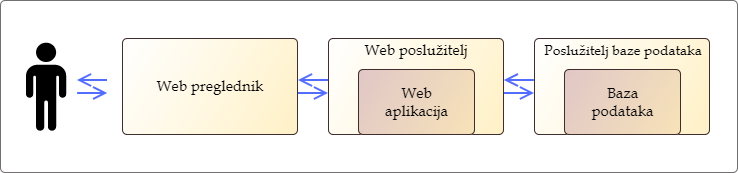
\includegraphics[width=\textwidth]{slike/arhitekturaSustava.png} %veličina slike u odnosu na originalnu datoteku i pozicija slike
	\centering
	\caption{Arhitektura sustava}
	\label{fig:arhitekturasustava}
\end{figure}

\textnormal{\textbf{Web preglednik} omogućava korisniku prikaz web stranice koja pruža određene funkcionalnosti. Omogućava prikaz web stranice (prikaz videa, slika i ostalog multimedijalnog sadržaja) onako kako je definirana u datotekama, dakle omogućuje interpretiranje koda u koristan oblik "običnom" korisniku.
	Putem web preglednika korisnik šalje zahtjev za željenu radnju koja se onda proslijedi idućim koponentama na obradu, te nakon obrade opet se prikazuju u vidljivom obliku kao vid povratne informacije.}

\textnormal{\textbf{Web poslužitelj} je ključna komponenta u obradi korisničkih zahtjeva.
	Dakle, to je \textbf{središnji dio} aplikacije koji omogućava komunikaciju korisnika s aplikacijom.
	U središnjem sloju se odvijaju procesi koji su zaslužni za komunikaciju s bazom podataka ukoliko je to potrebno,
	a to se odvija putem kontrolera, servisa i pristupu bazi podataka.
	U ovom sloju za komunikaciju koristi se Java programski jezik. Odnos komponenti predstavljen je slikom ispod.}

\begin{figure}[H]
	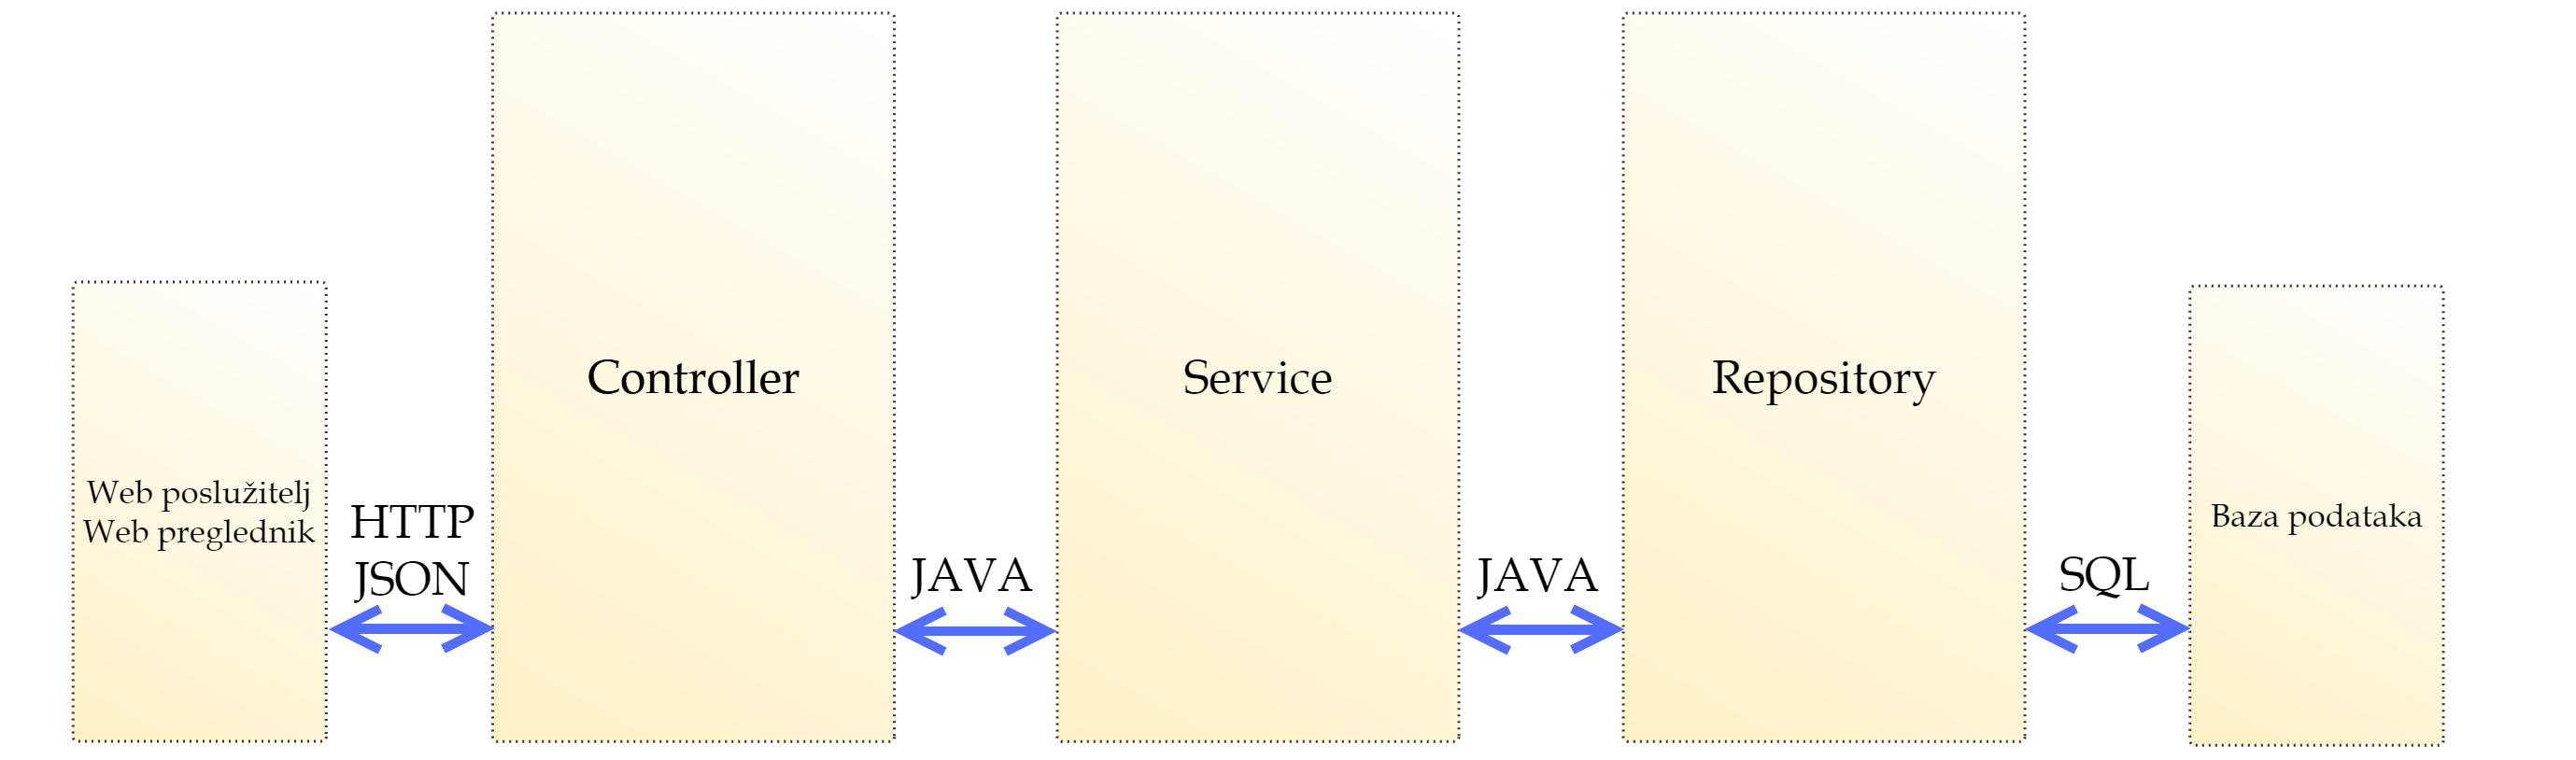
\includegraphics[width=\textwidth]{slike/arhitekturaSustava2.png} %veličina slike u odnosu na originalnu datoteku i pozicija slike
	\centering
	\caption{Arhitektura sustava backend}
	\label{fig:arhitekturasustava2}
\end{figure}

\textnormal{Za izradu ovakve web aplikacije kako bi se pokrile navedene specifične funkcionalnosti koristit će se Spring framework za Javu, te React za prikaz na web pregledniku u radnom okruženju IntelliJIDEA.
	Specifično za Spring framework, koristit će se navedeni tip arhitekture kao što je naveden slikom iznad, jer će se putem metoda JPARepository moći upravljati zahtjevima korisnika koji se vežu za upite u bazi podataka.
	Ukratko, obavljaju se operacije nad \textbf{bazom podataka H2}.}

\textnormal{\textbf{Kontroler} upravlja korisničkim zahtjevima i prosljeđuje ih dalje prema \textbf{Service} gdje se obavlja logika nad upitima i zahtjevima. Service komunicira s \textbf{bazom podataka} preko JPARepository.}

\textnormal{UI će biti povezan sa ostalim dijelovima web aplikacije putem \textbf{REST servisa}, odnosno REST servis komunicira s navedena tri sloja: Controller, Service i Repository. Takva vrsta komunikacije je predstavljena idućom slikom.
	UI je izveden uz pomoć \textbf{React} framework-a koji se koristi komponentama za organizaciju prikaza.}

\begin{figure}[H]
	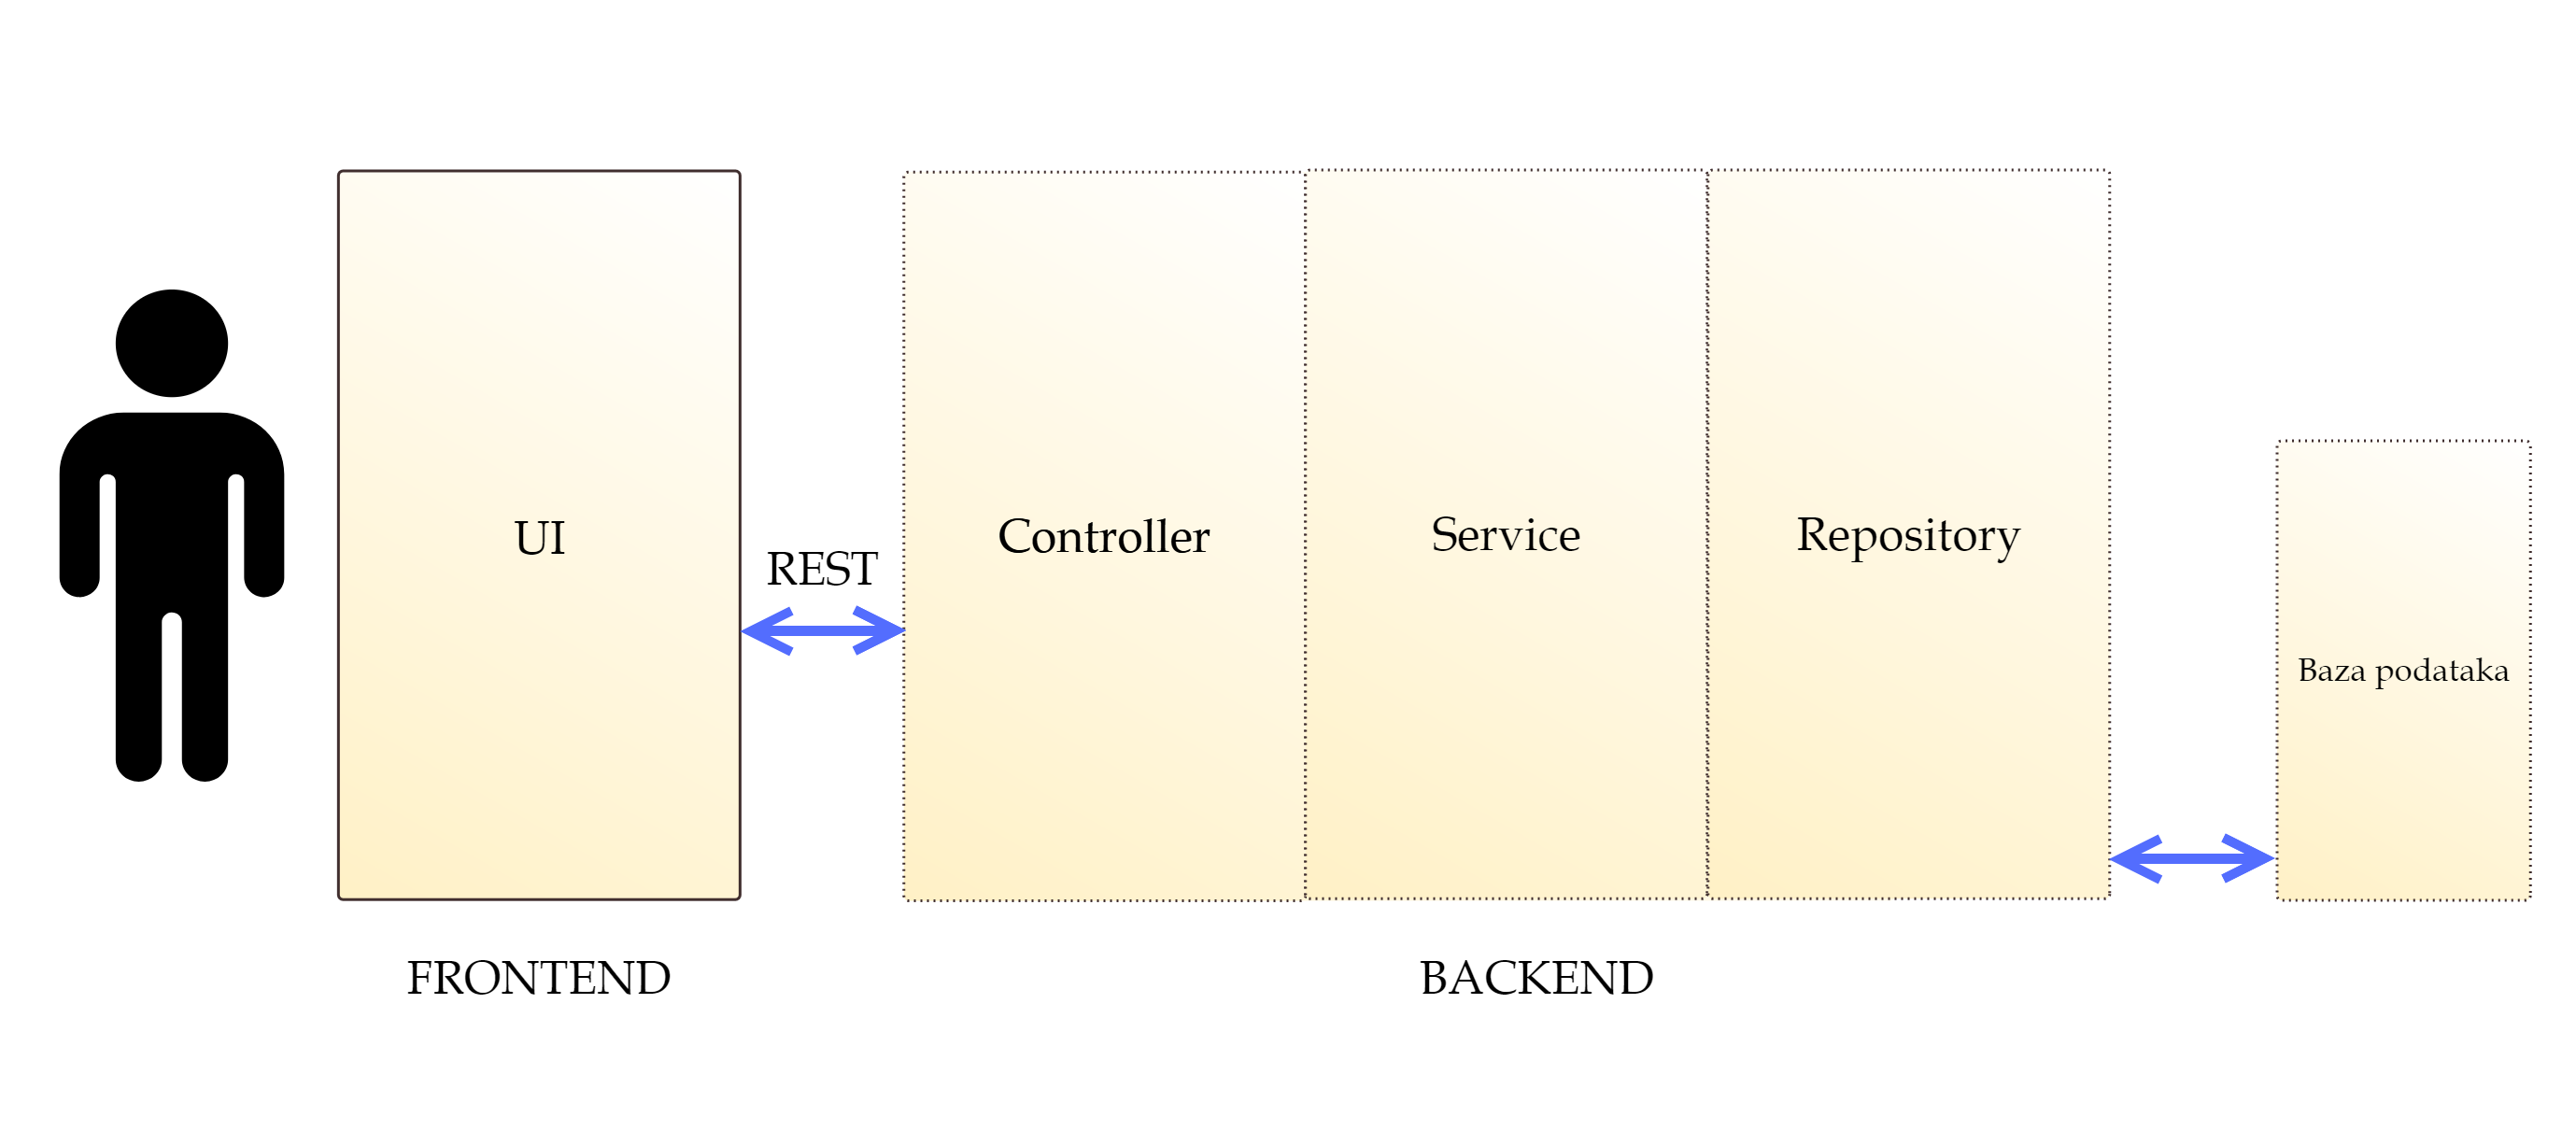
\includegraphics[width=\textwidth]{slike/arhitekturaSustava3.png} %veličina slike u odnosu na originalnu datoteku i pozicija slike
	\centering
	\caption{Arhitektura sustava backend i frontend}
	\label{fig:arhitekturasustava3}
\end{figure}

\eject





\section{Baza podataka}


\textnormal{Kao rješenje za web aplikaciju koju izrađujemo, odlučili smo se na relacijski model baze podataka jer nam ona omogućava precizno oblikovanje i modeliranje elemenata iz stvarnog svijeta. Međusobni odnos tablica se zasniva na relaciji dok se svaka tablica sastoji od naziva entiteta te njegovih pripadajućih atributa koji opisuju dani entitet. Ovakav tip baze podataka u ovom slučaju nam omogućava brzo spremanje, dohvat i izmjenu (uređivanje ili brisanje) podataka koji cirkulišu u web aplikaciji. Baza podataka koja je spremna za izradu ove web aplikacije se sastoji od sljedećih elemenata/tablica:}

\begin{packed_item}

	\item Korisnik
	\item Recept
	\item Video
	\item Objava
	\item Kategorija
	\item ReceptKategorije
	\item ReceptSastojci
	\item Sastojak
	\item Komentar
	\item OmiljeniAutor
	\item OznačenRecept
	\item SpremljenRecept
	\item VrstaKuhinja
	\item Obavijesti

\end{packed_item}

\eject

\subsection{Opis tablica}


				\textit{Svaku tablicu je potrebno opisati po zadanom predlošku. Lijevo se nalazi točno ime varijable u bazi podataka, u sredini se nalazi tip podataka, a desno se nalazi opis varijable. Svjetlozelenom bojom označite primarni ključ. Svjetlo plavom označite strani ključ}
				
				
				\begin{longtblr}[
					label=none,
					entry=none
					]{
						width = \textwidth,
						colspec={|X[6,l]|X[6, l]|X[20, l]|}, 
						rowhead = 1,
					} %definicija širine tablice, širine stupaca, poravnanje i broja redaka naslova tablice
					\hline \SetCell[c=3]{c}{\textbf{korisnik - ime tablice}}	 \\ \hline[3pt]
					\SetCell{LightGreen}IDKorisnik & INT	&  	Lorem ipsum dolor sit amet, consectetur adipiscing elit, sed do eiusmod  	\\ \hline
					korisnickoIme	& VARCHAR &   	\\ \hline 
					email & VARCHAR &   \\ \hline 
					ime & VARCHAR	&  		\\ \hline 
					\SetCell{LightBlue} primjer	& VARCHAR &   	\\ \hline 
				\end{longtblr}
				
				
			
			\subsection{Dijagram baze podataka}
				\textit{ U ovom potpoglavlju potrebno je umetnuti dijagram baze podataka. Primarni i strani ključevi moraju biti označeni, a tablice povezane. Bazu podataka je potrebno normalizirati. Podsjetite se kolegija "Baze podataka".}
			
			\eject
			
			
		\section{Dijagram razreda}
		
			\textit{Potrebno je priložiti dijagram razreda s pripadajućim opisom. Zbog preglednosti je moguće dijagram razlomiti na više njih, ali moraju biti grupirani prema sličnim razinama apstrakcije i srodnim funkcionalnostima.}\\
			
			\textbf{\textit{dio 1. revizije}}\\
			
			\textit{Prilikom prve predaje projekta, potrebno je priložiti potpuno razrađen dijagram razreda vezan uz \textbf{generičku funkcionalnost} sustava. Ostale funkcionalnosti trebaju biti idejno razrađene u dijagramu sa sljedećim komponentama: nazivi razreda, nazivi metoda i vrste pristupa metodama (npr. javni, zaštićeni), nazivi atributa razreda, veze i odnosi između razreda.}\\
			
			\textbf{\textit{dio 2. revizije}}\\			
			
			\textit{Prilikom druge predaje projekta dijagram razreda i opisi moraju odgovarati stvarnom stanju implementacije}
			
			
			
			\eject
		
		\section{Dijagram stanja}
			
			
			\textbf{\textit{dio 2. revizije}}\\
			
			\textit{Potrebno je priložiti dijagram stanja i opisati ga. Dovoljan je jedan dijagram stanja koji prikazuje \textbf{značajan dio funkcionalnosti} sustava. Na primjer, stanja korisničkog sučelja i tijek korištenja neke ključne funkcionalnosti jesu značajan dio sustava, a registracija i prijava nisu. }
			
			
			\eject 
		
		\section{Dijagram aktivnosti}
			
			\textbf{\textit{dio 2. revizije}}\\
			
			 \textit{Potrebno je priložiti dijagram aktivnosti s pripadajućim opisom. Dijagram aktivnosti treba prikazivati značajan dio sustava.}
			
			\eject
		\section{Dijagram komponenti}
		
			\textbf{\textit{dio 2. revizije}}\\
		
			 \textit{Potrebno je priložiti dijagram komponenti s pripadajućim opisom. Dijagram komponenti treba prikazivati strukturu cijele aplikacije.}